

\part[Mental arithmetic]{Mental Arithmetic}\label{c:mental}

\chapter[Memory for arithmetic facts]{Memory for Arithmetic
Facts}\label{c:xlit}

There are a number of ways to find the answer to ``\x67''.  Strategies
might include counting a row of six 7s, recalling the answer to \x66 and
adding on another 6, using a calculator, or pure recall. Children tend to
use a number of strategies, but as they become older they tend
to rely on recall alone \cite{siegmult}.

This chapter investigates adults' recall of multiplication facts.
Although adults do use other strategies, recall seems to be most frequently
used, and it is also the strategy that has been the subject of many
detailed experiments. First, a review is presented of the typical reaction
times (RTs) and errors of adults recalling multiplication facts.  A number
of models have been proposed to account for the phenomena, and these are
reviewed in section~\ref{s:xprevmod}.  A new connectionist model of fact
recall, based on \citeauthor{mccascade}'s \citeyear{mccascade,pdp3}
``cascade''
equations, is described in chapter~\ref{c:xnet}.



\section{Phenomena}

When asked to recall answers to single-digit multiplication problems, both
children and adults exhibit well documented patterns of behaviour. These
behaviours are recorded from experiments based around three kinds of task:
production, verification, and primed production.  In the production task,
subjects are presented with two digits and asked to recall the product.
The primed production task is similar to the production task, but before
the two digits are presented, the subject is shown a number which may or
may not be the correct answer to the problem.  For the verification task
the subject is presented with a problem and candidate solution
(``\xeq{6}{7}{48}?'') and
has to
decide if the equation is true or false.
In all cases, errors and RTs are recorded.

As production is the every-day task that subjects are familiar with, it is
the one that is considered here.  Many of the
experimental results come from normal subjects
\cite<e.g.,>{camp85,millcogn,camprole,ashcdeve,siegmult,harlasso,kruewhy}.
However, there are interesting results from brain-damaged subjects
\cite{mcclfact,sokocogn,mcclcogn}, and these are considered in
section~\ref{s:brainlit}.

\subsection{The production task}

Typical production experiments \cite<e.g.,>{camp85} run as follows: a
subject is seated in front of a computer screen on which two digits will
appear.  The subject is asked to respond ``as quickly and accurately as
possible'' when the digits are shown.  The RT is recorded along
with any errors the subject makes.  Usually only the problems from \x22 to
\x99 are tested.  In some experiments \x00 to \x99 is tested, although zero
and ones problems are often assumed to be solved by a separate mechanism.
The complications added by zero and ones problems are discussed later.

\begin{fancyfigure}
\centerline{\psfig{file=humanrt.ps,height=10cm}}
\caption{Plot of mean correct RT per multiplication table collapsed over
operand order for mean RT of: 60 adults \protect\cite[appendix~A]{camp85};
26 children in grade 5 (ibid.,~appendix~B).}
\label{f:humanrtplot}
\end{fancyfigure}

%%%%%%%%%%%%%%%%%%%%%%%%%%%%%%%%%%%%%%%%%%%%%%%%%%%%%%%%%%%%%%%%%%%%%%%%

\subsubsection{Reaction time}

In general, RTs increase across the multiplication tables. That is,
problems in the nine times table tend to take longer to answer than
problems in the two times table. However, this ``problem-size effect'' has
exceptions:
\begin{itemize}
\item The five times table is much faster than its position would suggest.
\item ``Tie'' problems (\x22, \x33 etc.)\ are recalled relatively quickly.
\end{itemize}

Figure~\ref{f:humanrtplot} shows the RTs
of adults and grade~5 children for
the eight multiplication tables, 2--9.  Overall, the developmental trend is
for a flattening of the RT curve, and a increase in response speed.  Note
that for the grade 5 subjects there is a noticeable dip in RT for the nine
times table which is not present for adults.  Zero and ones problems are
considered later (section~\ref{s:ruleslit}).


\begin{fancytable}
\tabcolsep=2.2pt\scriptsize
\renewcommand{\arraystretch}{0.625}
\begin{tabular}{lrrrrrrrrrrrrrrrrrrrrrrrrrrrrrrr}
&4&6&8&9&10&12&14&15&16&18&20&21&24&25&27&28&30&32&%
35&36&40&42&45&48&49&54&56&63&64&72&81\\
2$\times$2&c&&&&&&&&&&&&&&&&&&&&&&&&&&&&&&\\
2$\times$3&&c&&&&&&&&&&&&&&&&&&&&&&&&&&&&&\\
3$\times$2&&c&&&&1&&&&&&&&&&&&&&&&&&&&&&&&&\\
2$\times$4&1&1&c&&1&1&1&&&&&&&&&&&&&&&&&&&&&&&&\\
4$\times$2&&&c&&&2&&&1&&&&&&&&&&&&&&&&&&&&&&\\
2$\times$5&&&&&c&1&&2&&&1&&&&&&&&&&&&&&&&&&&&\\
5$\times$2&&&&&c&2&&&&&&&&&&&&&&&&&&&&&&&&&\\
2$\times$6&&3&&&&c&&&&2&&&&&&&&&&&&&&&&&&&&&\\
6$\times$2&&1&&&&c&&&1&&&&&&&&&&&&&&&&&&&&&&\\
2$\times$7&&&&&&1&c&&&1&&2&&&1&&&&&&&&&&&&&&&&\\
7$\times$2&&&&1&&2&c&&1&1&&&&&&&&&&&&&&&&&&&&&\\
2$\times$8&&&&&&1&1&&c&8&&&&&&&&&&&&&&&&&&&&&\\
8$\times$2&&&&&&2&1&&c&3&&&&&&&&&&&&&&&&&&&&&\\
2$\times$9&&&&&&&&&&c&&&&&&&&&&&&&&&&&&&&&\\
9$\times$2&&&&&&&&&2&c&&&&&&&&&&&&&&&&&&&&&\\
3$\times$3&&5&&c&&&&&&&&&&&&&&&&&&&&&&&&&&&\\
3$\times$4&1&&&&&c&&&&&&&&&&&&&&&&&&&&&&&&&\\
4$\times$3&&&&&&c&&&&&&&&&&&&&&&&&&&&&&&&&\\
3$\times$5&&&&&&&&c&&&&&&1&&&1&&&&&&&&&&&&&&\\
5$\times$3&&&&&&&&c&&&&&&&&&&&&&&&&&&&&&&&\\
3$\times$6&&&&1&&2&&&1&c&&&&&&&&&&2&&&&&&&&&&&\\
6$\times$3&&&&&&2&&&&c&&2&2&&1&&&1&&&&&&&&&&&&&\\
3$\times$7&&&&&&&&&&&&c&&&4&&&&&&&&&&&&&&&&\\
7$\times$3&&&&&&&1&&&&&c&&&1&&&&&&&&&&&&&&&&\\
3$\times$8&&&&&&&&&2&10&&1&c&&1&&&&&&&&&&&&&&&&\\
8$\times$3&&&&&&&&&1&5&&&c&&3&&&1&&&&&&&&&&&&&\\
3$\times$9&&&&2&&&&&&8&&7&1&&c&&&&&1&&&&&&&&&&&\\
9$\times$3&&&&&&&&&&13&&4&1&&c&&&&&2&&&&&&&&&&&\\
4$\times$4&1&3&&&&2&&&c&2&&&1&&&&&&&&&&&&&&&&&&\\
4$\times$5&1&&&1&1&&&&&&c&&&&&&&&&&1&&&&&&&&&&\\
5$\times$4&&&&1&1&&&&&&c&&&&&&&&&&&&&&&&&&&&\\
4$\times$6&&&&&&&&&&&&&c&&&1&&&&2&&&&&&&&&&&\\
6$\times$4&&&&&&&&&&&&&c&&&1&&&&&&&&&&&&&&&\\
4$\times$7&&&&&&&&&&&&3&3&&1&c&&1&&&1&&&&2&&&&&&\\
7$\times$4&&&&&&&&&&&&&6&&&c&&&&2&&1&&1&&&&&&&\\
4$\times$8&&&&&&&&&&&&&15&&&3&&c&&5&&&&4&&&&&&&\\
8$\times$4&&&&&&&&&&&&&20&&&2&&c&&&&2&&&&&&&2&&\\
4$\times$9&&&&&&&&&&&&&1&&2&&&4&&c&1&&&&2&&&&&&\\
9$\times$4&&&&&&&&&&&1&&1&&3&5&&1&&c&&&&&&&&&&&\\
5$\times$5&&&&&&&&&&&&&&c&&&&&3&&&&&&&&&&&&\\
5$\times$6&&&&&&&&&&&&&&1&&&c&&3&1&&&&&&&1&&&&\\
6$\times$5&&&&&&&&&&&&&&&&&c&1&5&&1&&&&&&&&&&\\
5$\times$7&&&&&&&&&&&&&&&&&1&1&c&&&1&4&&&1&1&&&&\\
7$\times$5&&&&&&&&&&&&&&&&&2&&c&&&&2&&&&&&&&\\
5$\times$8&&&&&&&&&&&1&&&1&&&&&2&&c&&3&1&&&1&&&&\\
8$\times$5&&&&&&&&&&&&&&&&&2&&2&&c&&4&&&&&&&&\\
5$\times$9&&&&&&&&&&&&&&&&2&&&3&&6&&c&&1&5&&&&&\\
9$\times$5&&&&&&&&&&&&&&&&&&&2&&4&&c&&&1&&&&&\\
6$\times$6&&&&&&&&&&&&&1&&&&&&&c&1&1&&&&&&1&1&&\\
6$\times$7&&&&&&&&&&&&&&&&1&&6&&2&1&c&&&&1&1&2&&&\\
7$\times$6&&&&&&&&&&&&&1&&&1&&4&&5&&c&&&&&2&1&1&&\\
6$\times$8&&&&&&&&&&&&&&&&&&&&&1&11&&c&&&&&1&&\\
8$\times$6&&&&&&&&&&&&&&&&&&&&&1&4&1&c&&4&5&&2&&\\
6$\times$9&&&&&&&&&&&&&&&&&1&1&&3&&1&2&&&c&9&10&2&3&\\
9$\times$6&&&&&&&&&&&&&&&&&1&&&11&&3&2&&2&c&10&2&&&\\
7$\times$7&&&&&&&&&&&&1&&&&&&1&&&&6&&&c&&&&&&\\
7$\times$8&&&&&&&&&&&&&&&&&&&&&&6&&7&&4&c&2&1&3&\\
8$\times$7&&&&&&&&&&&&&&&&&&&&&&4&&4&&6&c&&1&2&\\
7$\times$9&&&&&&&&&&&&&&&&&&&&1&&2&1&1&9&3&12&c&&2&\\
9$\times$7&&&&&&&&&&&&&&&2&&&&&3&&1&&&&4&8&c&1&5&\\
8$\times$8&&&&&&&&&&&&&&&&&&&&3&&&&1&&&1&2&c&&7\\
8$\times$9&&&&&&&&&&&&&&&1&&&&&&&1&&&&1&4&4&&c&3\\
9$\times$8&&&&&&&&&&&&&&&&&&&&&&&&1&&1&1&&&c&3\\
9$\times$9&&&&&&&&&&&&&&&&&&&&1&&&&&&&&&&&c\\
\end{tabular}
\caption{Error matrix for 60 subjects
\protect\cite[appendix~A]{camp85}.  Each element represents
the number of times a product occurred as an incorrect
answer to the corresponding problem (c = correct).
Given a total of 8640 trials (each subject tested on 4
blocks of 36 problems),
and an error rate of 7.65 per cent, it
appears that each ``c'' in the table corresponds to an average of 125
correct recalls.
In addition
to the errors shown here, \protect\citeauthor{camp85} labelled
17 errors
above \x54 as involving products less than 20.}
\label{f:errmat}
\end{fancytable}





%%%%%%%%%%%%%%%%%%%%%%%%%%%%%%%%%%%%%%%%%%%%%%%%%%%%%%%%%%%%%%%%%%%%%%

\subsubsection{Errors}

\citeA{camp85} found that adults under mild time pressure make errors at
the rate of 7.65 per cent.  These errors are distributed as shown in
table~\ref{f:errmat}.  Errors tend to be clustered around the correct
product.  More specifically, the errors can be classified as follows
\cite<after>{mcclmode}:




\begin{itemize}

\item Operand errors, for which the erroneous product is correct for a
problem that shares a digit (operand) with the presented problem. For
example, \xeq{8}{8}{40} is an operand error because the problem shares
an operand, 8, with \xeq{5}{8}{40}.

\item Close operand errors, a subclass of operand errors, where the
erroneous product is also close in magnitude to the correct product. That
is, for the problem $a\times b$, the error will often be correct for the
problem ($a\pm2) \times b$ or $a \times (b\pm2)$. An example is
\xeq{5}{4}{24}. This phenomenon is referred to as the ``operand distance
effect''.

\item Frequent product errors, where the error is
one of the five products 12, 16, 18, 24 or 36.  These products happen to
occur more frequently than most in the multiplication table
defined over integer operands from 2 to 9.

\item Table errors, where the erroneous product is the correct answer to
some problem in the range \x22 to \x99, but the problem does not share any
digits with the presented problem (e.g., \xeq{4}{5}{12}).

\item Operation errors, where the error to $a\times b$ is correct for
$a+b$.  These errors occur even in blocks of problems
which only contain multiplication problems.  Hence, it is unlikely that
they are only the result of a perceptual slip \cite{winkasso}.

\item Non-table errors, when the answer is not a product found in the
multiplication table.  For example, \xeq{4}{3}{13} is a non-table error
because
13 is not a number found in the multiplication table defined over \x00 to
\x99.  In the \citeauthor{camp85} study, only 7.4 per cent of errors were
in this category, and they are not shown in table~\ref{f:errmat}.
\end{itemize}
The main error categories are summarized in figure~\ref{f:sliptypes}.

\begin{fancyfigure}
\centerline{\psfig{file=xtable.ps,height=7cm}}
\caption{Slip categories.  Note that \xeq{4}{3}{13} is a non-table error
because
the number 13 does not appear as a product in this table.}
\label{f:sliptypes}
\end{fancyfigure}

Table~\ref{f:menterrorpc} summarizes the distribution of errors shown in
table~\ref{f:errmat}.  For comparison, the results from a similar
study by \citeA{harlasso} are also shown.
The statistics for the \citeauthor{harlasso} column, apart from error
frequency, were recomputed from \citeA[appendix~B]{harlasso}. As can be
seen from the table, most errors are operand errors, and more specifically,
close operand errors. Both studies agree on this, but note the difference
in the operation errors row. Harley's study included the \x00 to \x99
problems for which there are numerous errors of the form \x{0}{N}=N.
Approximately 11 per cent of the errors were \x{0}{N}=N errors, and these
have been classified as operation confusion errors in
table~\ref{f:menterrorpc}.

The RT and errors are tied together by \citeauthor{camprole}'s
\citeyear[p.~110]{camprole} observation
that there is a strong correlation of 0.93 between error rate and RT\@.
That
is, the problems on which a
subject is slowest are also the problems that the subject often gets
wrong.

\def\notedag{$^\dag$}
\setdec 00.0

\begin{fancytable}
\begin{center}
\begin{tabular}{l|cc}
\multicolumn{1}{c}{}& \multicolumn{1}{c}{Campbell} & Harley\\
\multicolumn{1}{c}{}& \multicolumn{1}{c}{\& Graham} & \\
\hline
Operand errors          &\dec 79.1 &\dec 86.2 \\
Close operand errors    &\dec 76.8 &\dec 76.74 \\
% Frequent product errors\notedag & \dec 30.6  &\dec 26.99 \\
Frequent product errors & \dec 24.2  &\dec 23.26 \\
Table errors            &\dec 13.5 &\dec 13.8 \\
Operation error         &\dec 1.7  &\dec 13.72 \\
Error frequency         &\dec 7.65  &\dec 6.3
%Error frequency         &\dec 7.65  &\dec 6.3 \medskip\\
%\multicolumn{3}{l}{\dag Percentage of operand errors.}
\end{tabular}
\end{center}
\caption{Percentage breakdown of errors. Figures are mean values for
sixty adults tested on \x22 to \x99 from
\protect\citeA[appendix~A]{camp85}, and 42 adults tested on \x00 to \x99
from \protect\citeA[appendix~B]{harlasso}.
For the \protect\citeauthor{camp85}
data, the operand error and operation error
percentages are an
approximation due to incomplete data.}
\label{f:menterrorpc}
\end{fancytable}


%%%%%%%%%%%%%%%%%%%%%%%%%%%%%%%%%%%%%%%%%%%%%%%%%%%%%%%%%%%%%%%%%%%%%%%
%\subsection{The verification and primed production tasks}
%%%%%%%%%%%%%%%%%%%%%%%%%%%%%%%%%%%%%%%%%%%%%%%%%%%%%%%%%%%%%%%%%%%%%%%

\subsection{Neuropsychological constraints}\label{s:brainlit}

Any good model of a cognitive skill should be structured in a way that is
similar to the equivalent human system.  Assuming that brain damage can
selectively impair parts of this structure, then it is reasonable to expect
that the model can be damaged to behave in ways that brain-damaged
individuals do.  That is, results from brain-damaged subjects suggest the
question: ``What must the normal system be like in order that, subsequent
to selective damage, performance breaks down in just the ways observed?''
\cite[p.~355]{sokocogn}.

Results from brain-damage studies \cite<e.g.,>{sokocogn,mcclfact} offer
further constraints on models, in addition to the empirical findings
reported above.

Brain damaged subjects, unlike normals, make a number of omission
errors, responding to problems with ``don't
know''. For example, \citeA[p.~177]{mcclfact}
report that two subjects failed to produce answers for 24 and 46 per cent
of trials.
On the trials where the subjects did produce incorrect answers, there was a
tendency for larger problems to show greater impairment than smaller
problems.  However, this impairment was
non-uniform. For
example, one subject (SB) had an error rate of 63 per cent on \x83 and
\x74, but was correct when answering \x86 and \x76.  The errors made tended
to follow the distribution discussed above: most of the errors were close
operand errors.




\subsection{Rule based processing}\label{s:ruleslit}

Figure~\ref{f:zerortgraph} shows the RT for
problems \x00 to \x99.
There are persistent statements in the literature that zero and one times
tables are governed by procedural rules. Evidence cited to support this
notion comes mostly from the relative RTs of zero problems. See, for
example, \citeA[p.~341]{camp85}; \citeA[p.~51]{millcogn};
\citeA[p.~334]{staznetw}.

However, the most persuasive arguments for a separate mechanism for zeros
and ones problems comes from studies involving brain-damaged subjects.
\citeA{sokocogn} reports that one patient (PS) showed errors
of \xeq{0}{N}{N} on almost all \x0N problems, and then suddenly improved to
almost perfect performance on all the zeros
problems (p.~358).  That is, unlike
other problems, zero problems show uniform impairment.

Further support comes from remediation studies \cite[p.~186--7]{mcclfact}.
Patient JG was trained on the problems
\x08, \x09, and some non-zero problems,
including \x27.  Although training on \x27 leads to improvement on \x72, JG
was correct on only 5
out of 355 problems that were not trained on.  In stark
contrast is the generalization on zero problems: after training on two
zeros problems, JG was 99.3 per cent correct on all other untrained zero
problems (139 of 140 problems correct). Similar remediation results suggest
that a rule \xeq{N}{1}{N} is also utilized.

Despite the convincing evidence for a rule-based mechanism,
it is not clear why certain errors occur
for zero problems. The majority of errors for zero problems take the form
of \xeq{0}{N}{N} \cite{harlasso}. \citeauthor{mcclfact}\ suggest two
explanations
for why these errors occur.

The first possibility is that the wrong rule is retrieved.  That is, when
presented with a \x0N problem, the subject attempts to retrieve the rule
\xeq{0}{N}{0} but actually finds 0+N=N or \xeq{1}{N}{N}.  However, it is
not clear why \xeq{0}{N}{N} errors occur for the problems \x01 and \x10.
In these cases, the rule \xeq{1}{N}{N} should be applied to give the
correct answer.

Another possible source of \xeq{0}{N}{N} errors could come from stored
incorrect rules.  That is, the subject stores a
rule like \xeq{0}{N}{N} alongside the correct rule.
\citeauthor{mcclfact}\ offer a scenario for how
such rules are acquired:  the incorrect rule \xeq{0}{N}{N} is a
generalization of the rule learned from addition, 0+N=N. The
generalization is: any operation involving zero and N results in N.
Ordinarily the
correct rule
will be used either because it was the most
recently learned rule, or because
it is the most specific rule.  The problem then is how brain-damage and
normal forgetting can lead to the selection of the incorrect rule in
preference to the correct rule.  One account is that ``\ldots the correct
rule [\xeq{0}{N}{0}] seems
essentially arbitrary to many individuals, where as the
incorrect rule seems to fit better with other knowledge of arithmetic. In
other words, to some individuals the incorrect rule may make more sense
than the correct rule'' \cite[p.~192]{mcclfact}.


\citeauthor{mcclfact}\ conclude that, although the account of rule-based
arithmetic is speculative, arithmetic recall is characterized as an
associate network of facts for 2--9 problems, augmented with rules
used for zero and ones problems. However, the problem is that no
models have been produced which incorporate rule-based processing together
with recall from an associative network.  Such a system needs to be built
to articulate the details of rule-based recall.
Also, it is not yet clear exactly what constitutes a rule
\cite{kirswhen,clarasso}. Given these
uncertainties, it may be worth first pursuing single mechanisms models to
account for the rule-like behaviour. This is further discussed in
section~\ref{s:rulesres}.

\begin{fancyfigure}
\centerline{\psfig{file=humanrt01.ps,height=10cm}}
\caption{Plot of mean correct RT per multiplication table collapsed
over operand order for: median RT of 42 adults
\protect\cite[appendix~D]{harlasso};
median RT (adjusted for naming time) of 6 adults
\protect\cite[table~A1]{millcogn}.}\label{f:zerortgraph}
\end{fancyfigure}



\subsection{Summary}

The major findings which constrain a model of arithmetic recall are:

\begin{enumerate}
\item The problem-size effect indicates that problems with large operands
tend to take longer to answer than problems with small operands.
\item There are exceptions to the problem-size effect, most notably the 5
times table and tie problems.
\item The majority of errors are operand errors, where the
incorrect answer is
correct for a problem that shares an operand with the presented problem.
\item Recall, when damaged, shows a pattern of non-uniform damage, rather
than a global degradation in performance.
\item Zero and ones problems appear to be rule-governed.
\end{enumerate}

Arithmetic is a well learned skill: a large number of individuals are
taught and ``know'' the times tables.  Yet some problems are easier than
others, and people do make occasional mistakes
when asked to recall these supposedly
well-learned facts.  What mechanisms capture the time-course of this skill,
and how are errors produced?  What kind of learning process installs these
mechanisms?


%%%%%%%%%%%%%%%%%%%%%%%%%%%%%%%%%%%%%%%%%%%%%%%%%%%%%%%%%%%%%%%%%%%%%%%%%

\section{Previous models}\label{s:xprevmod}

Various approaches have been taken to modelling the above phenomena.
Examples included: counting models, sometimes called digital models;
analogue models; network models; and procedural models, based around
rules for arithmetic.

Counting models assume that adults have internalized children's counting
strategies. For example, one of the most successful
counting models is the MIN model \cite{groechron}. To add two numbers,
$n$ and $m$, two counters are postulated: the first is set equal to the
larger of the two numbers (say, $m$); the second is used to increment
the first counter $n$ times.  Hence, addition is achieved by repeated
incrementing, and the RT will be a function of the smaller (MIN) number.
Although this model is a good predictor of addition RT, there are
problems when the system is applied to multiplication.

No counting account has been proposed for multiplication, but
as \citeA{staznetw} note, there are some straightforward ways to extend
the model to multiplication.  The simplest scheme assumes
that the first counter is set to zero, and then incremented by the
larger number, $m$, for a total of $n$ times.  However, this proposal
requires that the subject be able to count
not only in 1s, but also 2s, 3s, etc, and that the size of the
increment should not effect the speed of counting.
\citeA[p.~47]{ashcment} note:
\begin{ssquote}
Since the counting model proposed for addition asserts that subjects
count in units of one, the suggestion that adults can count in units of
varying size when multiplying, but not when adding, lacks internal
consistency.
\end{ssquote}

In addition, confusions between addition and multiplication, namely operand
errors, also suggests a single system for both skills
\cite{winkasso,millcogn}, and this is something
difficult to capture in a
counting system.  One of the reasons for postulating the MIN model was
to capture the problem-size effect.  However, the counting model has
difficulties with the 5s and ties exceptions
to the problem-size effect.


Little progress has since been made with
counting models, and no detailed models of errors have been
proposed. Attention has been focussed on network models, and these are
discussed in this chapter \cite<see>[for a detailed review of counting
models and other approaches]{cornet}.

The set of network models include the most explicit models that exist.
Unlike the reconstruction of answers performed by counting models,
network models assume an associative memory structure.  Activation is
assumed to spreading between problems and answers nodes. An review of
network models is given by \citeA{mcclmode}.  Two of
these models are presented next.


\begin{fancyfigure}
\centerline{\psfig{file=doa.ps,width=11cm}}
\caption{The problem-to-answer representations for the distribution of
associations model. Line thickness depicts strength of association
\protect\cite<figure based on figure~3 from>{mcclmode}.}
\label{f:doa}
\end{fancyfigure}

% -----------------------------------------------------------------------
\subsection{Distribution of associations}\label{s:siegler}

One of the more interesting network models is the distribution of
associations (DOA) model proposed by \citeauthor{siegmult}
\cite{siegmult,siegsub,siegadd}. The model is an account of strategy
choice---why retrieval is used sometimes, and other methods, such
as repeated
addition, are used on other occasions.  The network of associations that
make up an adult's
multiplication memory is formed by the success and failures
of children's back-up strategies.

Each problem is connected to a set of candidate answers consisting of the
correct product plus some incorrect answers.  For adults it is assumed
that the strongest associations are to correct products (see
figure~\ref{f:doa}).  For children, however, the distribution of
associations will be ``flatter'', representing limited experience with
multiplication.

The recall process begins by randomly selecting a confidence criterion.
\citeA{siegmult} notes that ``\ldots even 1-year-olds often will not state
an answer that is suggested to them if they do not believe the answer is
correct.  Such resistance suggests that they possess a standard, akin to a
confidence criterion, for stating an answer'' (p.~261).

An answer for a presented problem is retrieved according to the strength
of the association between the problem and the answer: the stronger the
association, the more chance the answer has
of being selected. If the association to the proposed answer is stronger
than the confidence criterion, the answer is stated.  In the cases where
the strength falls below the confidence criterion, another answer is
selected. This loop continues until a maximum number of attempts has been
made (1, 2 or 3---a number randomly selected at the start of the retrieval
process).

If no answer has been stated after the maximum number of attempts, one of
two processes can, probabilistically, follow: sophisticated guessing, or
problem elaboration.

Sophisticated guessing is just another attempt at retrieval from the
associative network.  However, no comparison is made to the
confidence criterion: the answer is immediately stated.

For elaboration, the model ``writes down'' the problem. For
human subjects,
this is done with pencil and paper.  For the computer model, this is
implemented by temporarily boosting the strength of the associations by 5
per cent.  Another retrieval attempt is then made, and the answer stated if
it exceeds the confidence criterion---and this is more likely with newly
increased strengths. \citeA{siegmult} comments: ``The written elaboration
may itself be associated with possible answers to the problem'' (p.~261).
It is not clear why this elaboration would help given the
modular structure of arithmetic skills outlined in chapter~\ref{c:intro}.
That structure indicates that presentation form (visual Arabic numerals
or verbal) is
independent of the arithmetic fact store.  Nor is it obvious how increasing
associative strengths is equivalent to the writing down of a problem.

If no answer is given after elaboration, a back-up strategy is used. The
strategy presented by \citeauthor{siegmult} is repeated addition, where a
counter is incrementing by $n$, $m$ times for the problem $n\times m$.

\subsubsection{Reaction time}

RT is dependent on how many of the above stages were processed before an
answer was produced.  Problems produced by repeated counting have to have
passed through the recall stage and either elaboration or sophisticated
guessing.  \citeA[p.272]{siegmult} reports that the RTs produced by the
model can match those of children and adults.  The cause of this is
outlined below.

\subsubsection{Errors}

Errors can arise from either: retrieving an incorrect answer that happens to
exceed the confidence criterion; or from miscounting when using a back-up
strategy.  For miscounting, there is a fixed probability that a number is
added twice or skipped over.  Also, two numbers could be added incorrectly.
For example, on \x28, the model could produce $8+8=15$.  The frequency
of these
errors is proportional to the size of the number being added,  except for
5s problems which are added as accurately as 2s.  \citeauthor{siegmult}
reports that children are particularly accurate at adding 5s, hence the
exception.

\subsubsection{Learning}

Every time an answer is produced, the association between the problem and
answer is increased.  Due to (presumed) external reinforcement, the
increment is twice as much for correct answers than incorrect answers.

Initially, the associative strengths are small (0.01), so retrieval is
likely to fail, and the repeated counting strategy would be used.
The correct association will form after the problem had been presented a
number of times assuming that repeated counting usually produces the
correct answer.  As associations grow in strength, recall will succeed
more often, producing more correct answers in a shorter RT\@.  Hence,
the model accounts for the
development towards relying on recall and for RTs to decrease.

The problem-size effect is derived from the assumption that repeated
counting is more prone to errors on larger problems.  This is
seems likely because more addition steps are needed for larger problems.
So for larger
problems, repeated
counting will produce a distribution of associations that is ``flatter''
for large problems than small, resulting in longer RTs and more
errors.  Exceptions to the problem-size effect can be incorporated into the
model. An
example is the 5s problems discussed above for which the back-up
strategy reliably produces the correct answer, meaning that strong
associations will quickly form for these problems.

Problems are also presented according to the frequencies found in a school
textbook.  As smaller problems tend to be presented more often than larger
problems, this adds to the effect (discussed further in
section~\ref{s:presfreq}).

\subsubsection{Discussion}

\citeauthor{siegmult}'s DOA model is based on an associative network in
which problem nodes are linked to candidate answers. ``Associations across
arithmetic operations (e.g., addition and multiplication) are also
hypothesized to be present in the network'' (p.~259), but this is not
discussed in any detail by \citeauthor{siegmult}.

Operand errors are accounted for by the way the back-up strategy
miscounts.  When adding a group of 6s for the problem \x46, the strategy
may add one too many, resulting in 30, or one too few, 18.  Both are
operand errors.  Moreover, because the strategy is more likely to err
once, rather than twice or more, operand errors will be close to the
correct product.

The other way in which the back-up strategy can produce an incorrect answer
is by adding two numbers and getting the wrong result (e.g., $2+2=5$).  It
turns out, from \citeauthor{mcclmode}'s \citeyear{mcclmode} analysis,
that this behaviour will
produce more non-table errors than table errors.  This is the opposite of
the results reported by \citeA{camp85} for adults.
\citeauthor{siegmult} presumes
that counting errors will be distributed around the correct answer. That
is, the error \x67=41 (under counted by 1) and \x67=43 (over counted by 1)
occur more often than errors that result from larger miscounts. Given this
assumption, \citeauthor{mcclmode}\ note that for the 64 problems \x22 to
\x99, errors of the form $(n\times m)\pm1$ turn out to be non-table errors
twice as often as table errors. Hence, \citeauthor{siegmult}'s model
predicts the opposite of the observed situation, where table errors occur
twice as often as non-table errors for adults.

Although more explicit than many models, there are some details missing from
the DOA account.  For example, answers are retrieved from the associative
network with a probability proportional to associative strength.  This
aspect of the model is not fully elaborated: is it a spreading activation
system? If so, how does activation spread? By what mechanism are responses
selected? As will be shown later, many models have focused on just this
aspect of retrieval.

The model contains a number of separate mechanisms: recall, elaboration,
sophisticated guessing, and back-up.  No details were given about the
nature of the overall control mechanisms: what factors determine why
sophisticated guessing is used sometimes (20 per cent of trials), but
elaboration used at other times?  How and why is the associative strength
temporarily boosted for the elaboration stage?

The simulation results reported by \citeA{siegmult} were for just 20
problems due to limited resources, and this should be extended.

Finally, it is assumed that back-up strategies behave in the ways
specified. It would be interesting to see a more detailed account of the
structure of these strategies, explaining why they err in the ways that
they do.

The DOA model is an interesting account of strategy choice.  As a model of
recall of multiplication facts, it needs to be further specified.


% -----------------------------------------------------------------------

\begin{fancyfigure}
\centerline{\psfig{file=candg.ps,height=10cm}}
\caption{Network interference model.  Based on figure from
\protect\citeA{mcclmode}.}\label{f:candg}
\end{fancyfigure}

\subsection{Network interference}

\citeauthor{camp85}'s \citeyear{camp85} ``network
interference'' (NI) model does not
concern itself with multiple strategies as the \citeauthor{siegmult}
model does. Rather, just the associative retrieval component is
considered.

Figure~\ref{f:candg} shows the architecture of the model, which consists
of four kinds of units:
\begin{enumerate}
\item Operand units, to encode the 6 and 7 of \x67.
\item Problem units, activate only for specific problems.
\item Product units.
\item General magnitude units.
\end{enumerate}
Operand units are connected to the products in the operand's table. That
is, the operand unit 3, for example, is connected to the products 6, 9, 12,
15, and so on.  ``Type'' product units are used---there is only
one product unit representing 24, which is activated by \x46 and \x38.
The alternative to type product units is token units, in which there
would be two 24 units, one activated by \x46 and the other by \x38.

To disambiguate certain answers, a set of problem units are used.  For
example, with type product units, there is no way to choose between 32
and 24 when 8 and 4 are presented to the system: 32 is doubly activated
by the 4 and 8 in \x48; but 24 is also activated, once by the 8
(\xeq{3}{8}{24}),
and again by the 4 (\xeq{4}{6}{24}).
With problem units, the correct product will
receive an extra input.

Problem units also activate the magnitude units, which in turn activate an
appropriate set (large, medium, etc.)\ of product units. This allows the
subject to estimate the size of the answer.  Product units
that have answer digits in common---such as 12 and 15, or 12 and
32---are
connected together.

\subsubsection{Learning}

The NI model suggests that problem presentation frequency and order
determine the strengths of the associations in the network.
\citeA{camp85} assume that smaller problems are learned first, and are
presented more frequently, than larger problems. These assumptions are
not unreasonable, and chapter~\ref{c:xnet} looks in detail at
presentation frequencies.  However, for problem
frequency there is an inherent difficulty in discovering the actual
frequency experienced by subjects. \citeauthor{siegmult}'s results are
based around the frequency of problems from school textbooks, but
children certainly experience arithmetic problems other than those found
in textbooks.

Nevertheless, given the assumptions stated above, \citeauthor{camp85}
predict that the first problems learned will impair the learning of
later problems (proactive interference).  These smaller learned problems
will also act as a source of error for larger problems. That is, during
learning, the smaller problems will not have many alternative answers to
produce as an error.

\subsubsection{Errors}

Operand errors may occur because each operand unit is connected to a set
of product units.  On some occasions, the wrong product may be selected,
giving an operand error.  Close operand errors are produced because the
general magnitude units activate products that are approximately the
correct magnitude for the presented problem.

Errors also occur because of false associations. During learning, inputs
are associated with the correct
product.  However, due to the fact that activation spreads, other
product units will be active. Associations will also be made to these,
slightly active, false products.

Learning usually occurs in
lessons, where a number of problems will be presented and solved.
\citeauthor{camp85} argue that residual activation of problem units and
product units other than the one being solved will be associated with
the current problem. In this way, false associations are formed, which
may be produced as errors.  In particular, it is assumed that
problems close in magnitude (e.g., \x78 and \x79) are more likely to be
learned in the same lesson than more distant problems (such as \x78 and
\x72).  As \citeA{mcclmode} note, this suggestion is not
backed by any empirical evidence.  If true, it would further contribute
towards the production of close operand errors.

The connections between products
that share digits will produce some table errors, but this seems rather
``ad hoc---the associations between answers sharing a digit seem to
play no role in the model other than that of explaining certain table
errors'' \cite[p.~393]{mcclmode}.

As all the answers units correspond to a product, there is no account of
non-table errors.

\subsubsection{Retrieval}

One of the founding ideas behind the NI model is that the activation of
incorrect answers interferes with recall of the correct answer.  That
is, as interference increases, RT will become longer, and there will be
an increased chance of an error.

As mentioned, retrieval is a spreading activation process.  The
rules governing the spread of activity are not specified, and nor
is the response mechanism.  Presumably the most active product unit is
selected as the answer.  RT is assumed to be a function of
answer activity, but again, this is not specified.

\subsubsection{Discussion}

The lack of specific detail with this model (no activation rules, no
response mechanisms for correct or erroneous answers) is
not surprising given
that the system was not implemented.  As it stands the system is a
conceptual analysis of arithmetic and raises a number of questions:
\begin{itemize}
\item Why so many kinds of nodes?  What does each knowledge source
contribute to the model?  Are they all necessary?
\item How do these knowledge sources develop?   In particular, how are
the magnitude units formed?
\item How are problem-size exceptions handled?  Although
the system can accommodate exceptions, it would presumably have to be via
problem frequency or order.
\citeA{camp85} briefly comment on the
possibility of a rule-based system for 5s (the product should end in
zero or five), but do not pursue it in any depth.
\item By what means are the associations strengthened?  A brief
description was given, but without more specific learning mechanisms it
is not possible to determine the relative importance of each kind of
link.
\end{itemize}
The model itself lacks detailed mechanisms, but provides a useful source
of ideas for what factors may contribute to the phenomena.

% ====================================================================

\section{Previous connectionist models}

The rest of this chapter considers those models that are strongly
connectionist.  It seems apparent that connectionism is
appropriate for this task, and that the rigour of implementation could
flesh out some of the modelling issues introduced above.

The first connectionist account was built and developed by a group at Brown
University from 1989 onwards \cite{andestud,viscrepr,viscmemo,andeexpe}.
This account is unsatisfactory for reasons set out in
section~\ref{s:bsb}. \citeA{grahconn} also performed some experiments with
a connectionist network, but the model lacks an explicit recall mechanism.

No less than three other connectionist models were built in
answer to \citeauthor{mcclmode}'s call to ``shift from a demonstration of
the framework's basic merit to the hammering out of detailed, fully
elaborated models'' \citeyear[p.~394]{mcclmode}.  These models were
developed independently at more-or-less the same time. The first to be
published was the model by \citeA{mcclmath}, followed by the model
described in chapter~\ref{c:xnet} \cite{dallmemo,dallspee}. The most recent
model was built by \citeA{rickinte}.
The connectionist models are described below, and compared in the next
chapter.

% -----------------------------------------------------------------------

\begin{fancyfigure}
\centerline{\psfig{file=bsb.ps,height=7cm}}
\caption{BSB network.  This figure is a simplified picture
of the 1266 unit network described by
\protect\citeA{andestud}.}\label{f:bsb}
\end{fancyfigure}

\subsection{Brain-state-in-a-box}\label{s:bsb}

The brain-state-in-a-box (BSB) model
\cite{andestud,viscrepr,viscmemo,andeexpe} has been presented in a number
of forms.  Initially it was built for ``qualitative multiplication'', in
which answers are only ``ballpark estimates''.  That is, the model had a
small number of answers (e.g., \x31=5, \x32=5, \x62=10).
Most of the BSB simulations are of qualitative
multiplication, but \citeA{andestud} have started to model quantitative
multiplication.

The most recent simulations present a network with 1266
units.  The units are split into three groups (see figure~\ref{f:bsb}): two
sets of units for the two operands, and another for the answer. Each of
these three groups consists of two sets of units: a bar encoding of the
number, and an arbitrary symbolic label.

The bar encoding is the activation of a consecutive number of units.
That is, a number is encoded by
the positioning of the bar along the set of units,
forming an ``analogue'' encoding. The units are
arranged in an approximately logarithmic fashion, so that large numbers are
less distinct from each other than smaller numbers.

Originally, the symbolic component encoded the name of a number (e.g.,
``one'') based on the ASCII representation of characters.
\citeA{mcclmath} noted that this representation is unmotivated.  Problems
are usually encountered as Arabic numbers or spoken words, but almost never
as written words, such as ``eight times six''.  Yet, it was just this
spelling of the numbers that was used as input to the network.  It now
seems that the symbolic input is no longer supposed to represent the
spelling of a number, and is just presented as a random vector.  This input
still remains unmotivated, and it is not clear what purpose it serves in
accounting for the phenomena.

For each operand and answer there seems to be 150 units to
represent the symbolic and bar part.  From the reports on the system, it is
not clear how the units are divided up for each input field, or how wide
the bar is. This uncertainty is also commented upon by \citeA{mcclmath}.

The large number of units means that simulations require a large amount of
CPU time. Because of this, only 32--34 facts are trained.
In an attempt to scale the system to all the multiplication problems,
an extra field was added to the answer field.  This new field contains 60
units to encode nine ``integer symbols'' and ``\ldots tries to capture hazy
intuitions about two digit numbers having a most and least significant
digit'' \cite[p.~7]{andestud}.  No further details were given about this
new field: does it represent the ``tens'' or ``units'' part of the
answer? How does it affect recall?.

For training, the operand and answer units are clamped with desired
activations, and the weights between the units are adjusted using the
Widrow-Hoff error correction rule.  In previous simulations
\cite{viscrepr}, each problem was presented 30 times, in a random order.

\subsubsection{Recall}

When simulating recall, the operand units are clamped, and the answer units
compute their activation as follows:
$$
o_i(t+1)= \alpha \sum\limits_j w_{ij}o_j(t) + \gamma o_i(t) + \delta f_i(0)
$$
\noindent where: $o_i(t)$ is the output of unit $i$ at time $t$, which is
limited to be between $-1$ and $+1$; $\alpha$ is the feedback constant;
$\gamma$ is the decay constant; and $f_i(0)$ is the external input to the
unit, multiplied by a constant $\delta$.

The state of the system representing associations between operands and
answers forms an attractor.  The units in the network continue to update
until the system arrives at one of these point attractors. Cycling
continued until ``all of the vector elements were saturated''
\cite[p.~150]{viscrepr}.  That is, there was a read out threshold, and once
all the units had exceeded this threshold, processing stopped. The number of
cycles required to reach this point is taken as the RT for the presented
problem.  On some runs updating was stopped
when a maximum number of cycles (60) was reached.

\subsubsection{Reaction time}

\citeA{andestud} report that a number of their BSB simulations exhibit a
problem-size effect. The 32 simulated RTs reported in their paper do seems to
follow the problem-size effect. For this small sample of problems it
is not clear if there are exceptions for 5s, or if tie problems are
accounted for.

\citeauthor{andestud} agree with \citeauthor{camp85} that problem frequency
and order are important causes of the problem-size effect. It does not
appear that the BSB simulations make use of problem order or frequency,
although it is noted that: ``Practice and order effects are, of course,
easy to model within an associative framework'' (p.~13).

It is further suggested that the problem representation is also responsible
for the problem-size effect:
``\ldots the codings for problems of increasing magnitudes
may get successively more `muddled together'{''}.  However, ``\ldots it
does not appear that the problem-size effect resulting solely from the bar
code compression is a particularly robust feature of the modeling''
(p.~13).

\subsubsection{Verification}

With the architecture of the BSB model it is possible to study the
verification task. Distant false problems (such as ``\x52=60?'') and close
false problems (``\x52=20?'') were presented to the network by clamping
both operand and answer units. If, during processing, the network
overwrites the answer field, the problem is considered rejected.  If the
answer field remains unchanged, the problem is accepted. Simulations showed
that the network would reject distant products
faster than products that were close to the
correct product.  The system also accepted near false products, but no
distant false products.

\subsubsection{Errors}

Adults are quite capable of learning the multiplication facts, although
with some difficulty.  Any errors are, as \citeA{mcclmath} calls them,
occasional: errors in retrieval, and not predominantly errors resulting
from false beliefs. This is not the case for the BSB model.  The network,
as presented, is simply incapable of learning all the associations. For
example, on \x84 the network produced the answer 24 or 28, but never 32.
This runs against the notion that
slips are one-off run-time errors, rather than permanent disabilities.
Correct answers
are reconstructed for about 70 per cent of the problems.

The errors that are made are close in magnitude to the correct answer.
Examination of the results given in \citeA{andestud} shows that some of the
errors are close-operand errors, others are non-table errors. No details
are given on the proportions of the errors generally, or how
non-close operand, table or operation errors occur.

\subsubsection{Discussion}

Although there have been a number of papers describing the BSB model,
details of the model are still unexplained, and only small scale
simulations have been performed.  A number of points need to be clarified:
\begin{enumerate}

\item The motivation for the symbolic component of the representation, and
the role it plays in explaining the phenomena, is uncertain.

\item The details of the input representations (e.g., the ``roughly
logarithmic'' operand units) need to be given.

\item The 60 units used to encode ``integer symbols'' in the answer field
remain a mystery. What do they represent? What is the motivation for
it?

\item There is no account of occasional, run-time, errors.

\item The RT results do not cover ties, or the other exception to the
problem-size effect.

\item  The results from qualitative simulations are interesting, but what
bearing does this have on the multiplication done by people?

\end{enumerate}

\citeA{mcclmode} comment that the \citeA{viscrepr} ``proposal has several
limitations and cannot be considered a well-articulated model'', but add
that ``the [neural net] approach probably merits further exploration''
(p.~395).

% -----------------------------------------------------------------------
\subsection{Backpropagation}

\citeA{grahconn} has run a large number of simulations looking at how a
connectionist network can store arithmetic facts.  His model contained two
sets of input units to encode the two operands connected to a set of hidden
units.  The hidden units were connected to a set of output units divided
into tens and units fields.  Various parameters were explored, including:
number of hidden units; learning rates; input and output encodings; problem
presentation ordering; and rehearsal schedules detailing when
and how often trained
problems were re-presented.

A problem-size effect was found by training on small problems first. The
problems \x22 to \x99 were split between a large group (products
greater than 32)
and a small
group. Training with backpropagation on the small group first
produced a problem-size effect for the accuracy of the network. That
is, more smaller problems were correct than larger problems.

Errors were measured by testing the network at various stages during
learning, at 20 per cent correct and 70 per cent correct.  These errors
were mainly operand errors.

\citeauthor{grahconn}'s work cannot be considered as a model of the recall
process because it provides no explicit retrieval processes by which errors
and RTs can be measured. Nevertheless, it is a useful study, and suggests
that connectionist system may be useful in this domain.

% -----------------------------------------------------------------------

\begin{fancyfigure}
\centerline{\psfig{file=ia.ps,height=6cm}}
\caption{Interactive activation network
\protect\cite<from>[figure~5]{rickinte}.}\label{f:ia}
\end{fancyfigure}

\subsection{Interactive activation}

Like the BSB model, the interactive activation (IA) model proposed by
\citeA{rickinte} is a settling network.  The architecture of the network is
shown in figure~\ref{f:ia}.

There is just one set of input units to represent both operands.  Each
operand is connected, by a fixed weight, to every problem unit which
contains that operand.  The problem level is motivated by the success of
other associative memory models that use a part-whole hierarchy---such as
the interactive activation model of word perception,
\cite[chapter~7]{pdp3}.
At the problem level there is mutual inhibition (again, by a fixed value)
to implement the constraint that only one problem unit should be active.  A
set of type product units receive activation from, and send activation back
to, the problem units. There are also false associations between problem
units and product units. All the weights in the network are hand-crafted;
learning is not accounted for.

Processing begins when a problem is presented and the appropriate operand
units are clamping on.  A multiplication unit is also activated for all
problems, and presumably future extensions will include
units for addition, subtraction and division, too. The correct problem unit
will receive input
from three nodes (the two active operands
and the multiplication unit), and
table-related problem units will receive input from just two nodes (one of
the operand units and the multiplication unit).  Hence, the correct problem
unit will be most active, inhibiting other units, although table-related
problems will be slightly activated.

Note that for tie problems only one operand unit would be activated. This
means that tie problem units will only be activated by two inputs, as will
all the other problem units associated with the operand.  In order for the
correct problem unit to be activated, \citeauthor{rickinte}\ include a
``tie'' unit as part of the input.  This unit is activated whenever a tie
problem is presented, supplying the tie's problem unit with three inputs.
The motivation for the ties unit stems the notion that there is an ``\ldots
intrinsic uniqueness in the representations/processes\ldots that underlie
performance on these [tie] problems'' \cite[p.~18]{rickinte}.  That is,
there is ``something special'' about tie problems, and this is represented
by an extra bit on the input layer.

All the units in the IA network are updated synchronously.  The activation
of a unit is just the net input to the unit, but is never allowed to drop
below 0 or go above 1. Processing stops when a product unit exceeds a
threshold of 0.8.

As described so far, the system will always produce the correct response.
\citeauthor{rickinte}\ report that an incorrect
product units never exceed an activation of 0.1.
RT is the number of cycles it takes before a product unit exceeds the
threshold.  All problems reach threshold at the same time (after 43
cycles).

\subsubsection{Response times}

To explain the problem-size effect, \citeauthor{rickinte}\ hand modified
the problem-to-product weights.  It is assumed that the more frequently
occurring problems will cause stronger associations between units. To
implement this,
the problem set was split into two sets: ``small'' problems,
with products of 30 or less; and the remaining ``large'' problems.  Based
on the assumption that larger problems are experienced less often, the
weights between all units involved in the larger problems were decremented
by 10 per cent from the values given in figure~\ref{f:ia}.  After this
change 42 cycles were required for small problems, and 51 for the large
problems.

False associations are also assumed to interfere with retrieval.  To
simulate this, false connections were made between a problem and various
product units---one each for an operand error, close operand error,
table error, and non-table error.  The weights for the incorrect
associations were set at 0.025 for problem-to-product links,
and 0.0125 for
product-to-problem.  With the model modified in this way (independently of
the changes described above), cycle time increased to between 43 and 48
cycles.
Again, assuming that larger problems have
stronger false associations, \citeauthor{rickinte}\ state that false
associations can contribute to the problem-size effect.

\subsubsection{Errors}

Errors are only accounted for implicitly.  It is assumed that the
probability of an error occurring is proportional to the activation of the
product during cycling. As described above, the products
associated with operand errors and close operand errors are more active
during processing than table-unrelated products. Hence, given that more
active products are more likely to be errors, the IA model predicts more
frequent operand errors than table-unrelated errors.

\subsubsection{Primed production and verification}

The primed production task is simulated by activating the product node
corresponding to the prime, and allowing the network to cycle 6 times to
simulate brief exposure. Activation is then removed from the primed node,
and retrieval begins as described above.  When the correct node is primed,
the system's response is faster: 38 cycles compared to 43 without priming.
The IA system
slows when an incorrect prime is presented, and slows more when the
incorrect prime is related to the correct answer. When false associations
are included this increase in RT is even more
prominent. These results are consistent with those reported for human
subjects.

Similar results are reported for the verification task.  The verification
task is simulated like primed production, but leaving the candidate answer
mildly activated (external activation of 0.01) for the duration of the
experiment.  False problems slow the system, and this varies with the
degree of similarity between the correct and primed product.
Note that the system is not changed in any way to output
``yes'' or ``no'' in answer to the verification task. The answer is
selected by the mechanism described above.
Presumably, the decision as
to the
whether the candidate
product is correct or not, is a stage to be added after the production of a
product.

\citeA{rickinte} also introduce a verification strategy based on
``resonance'' as an alternative to the above method.
Resonance is defined as a global measure derived from
\citeauthor{pdp:6}'s \citeyear{pdp:6} ``harmony'' measure:

$$ \mbox{harmony} = \sum\limits_{ij} o_i o_j w_{ij} +
\sum\limits_i \mbox{ext}_i o_i $$


\noindent where $o_i$ is the output of unit $i$, $w_{ij}$ is the weight
between units $i$ and $j$, and ext$_i$ is the external input to unit $i$.
The harmony, or resonance, of the system, as defined here, will increase as
the ``self-consistency'' of the network increases.
That is, the correlations between active units connected
by strong positive weights increases.
During
verification tasks, \citeauthor{rickinte}\
show that harmony does increase
across cycles, and it increases faster with a correct candidate.  Harmony
increases slowly when an operand error candidate is presented, but
increases more quickly as the table-relatedness of the candidate is reduced
to table-unrelated candidates.  ``Thus, under the assumption that there
is a criterion resonance for responding `true', the probability of
responding `true'
incorrectly based on resonance in memory is greater when a
candidate answer is table-related and/or has an incorrect association to
the problem representation'' \cite[p.~28]{rickinte}.  There is no
discussion of how the global resonance measure is computed by the
system.

\subsubsection{Discussion}

The IA model has a general problem: there are too many assumptions, and not
enough quantitative simulations.  Indeed, it is not possible for
\citeauthor{rickinte}\
to produce many simulations without specifying some
more recall mechanisms.  In particular, there needs to be an explicit
account of error production. As \citeA[p.~88]{andearch} notes:

\begin{ssquote}
Activation does not directly result in behaviour.  At any point in time a
great deal of information may be active\ldots There must be processes that
convert this activation into behaviour.  A serious gap in much of the
theorizing about spreading activation is that these processes have not been
specified.
\end{ssquote}

This criticism applies directly to the IA model. It is not enough to assume
certain kinds of associations will form, or that error probability is
proportional to activation. It was already clear that
associative networks of many kinds \cite<e.g.,>{grahconn,viscrepr} could be
constructed to
account for some of the empirical observations on human behaviour.
As
\citeA{mcclmode} have commented,
network models show a great deal of promise
for this domain, but ``detailed, fully elaborated models'' are required.
The IA model lacks these details:

\begin{enumerate}

\item There is no learning mechanism.  As discussed above, the IA model has
a set of hand-crafted weights.  These weights are sometimes changed to
reflect assumptions about strong, weak or false associations.
But the point of interest is in exactly how the
distribution of weights is formed to conform to these assumptions.

\item The problem level in the IA model clearly plays an
important role, accounting for many of the interesting results.  However,
no account is given of why or how this particular representation should
develop.

\item  The assumptions about the distribution of associations are based on
the work of \citeA{siegmult}.  However, as described in
section~\ref{s:siegler}, there are problems with this account.

\item No detailed RT results are given.
One of the methods used to account for the problem-size effect
was to decrementing the weights of the ``large''
set of problems.  Does this mean that
only two different RTs could be generated, one for the small problems and
one for the large?  The other modification of adding
false associations was
done independently of the decrementing of weights, and it is not clear how
these two methods interact without a detailed comparison to human
human RT data.

\item No account is given for the speed of the tie and 5s problems.

\item No account is given  of zero- and one-times problems.

\item The IA model is particularly let down by the lack of an
explicit mechanism to account for incorrect retrieval.
Without a mechanism for this the system cannot actually produce errors,
regardless of internal
activity.

\end{enumerate}

It remains to be seen if the system can be modified to accommodate the
above.

\begin{fancyfigure}
\centerline{\psfig{file=mathnet.ps,width=12cm}}
\caption{Architecture of MATHNET \protect\cite<from>[figure~3]{mcclmath}.}
\label{f:mathnet}
\end{fancyfigure}


% -----------------------------------------------------------------------


\subsection{Mean field theory}

The most well-informed of all the connectionist models is
 MATHNET \cite{mcclmath}.  The architecture is
shown in figure~\ref{f:mathnet}, and is based around mean field theory
\cite[chapter~2]{hertintr} which is related to Boltzmann machines
\cite{pdp:7}.

The 26 problem nodes are divided in to
two groups of 12 nodes to encode the two operands, and 2 nodes to encode
the task---although only multiplication problems are currently considered.
The inputs
feed to 40 hidden nodes. The output layer consists of a set of 12 nodes to
encode the tens part of the answer, and another 12 to encode the
units field.
The output nodes are connected to each other. All weights in the
system are bidirectional.

Each operand is encoded as a bar of activity across three units. For the
operands 7, 8 and 9 the input pattern would be\ldots
\begin{verbatim}
  7:  - - - - - - - + + + - -
  8:  - - - - - - - - + + + -
  9:  - - - - - - - - - + + +
\end{verbatim}
\noindent\ldots where \verb|+| signifies an activation of $1.0$ and
\verb|-| signifies $-1.0$.  There are enough input units to encode the
operands 0 to 9, but only the problems \x22 to \x99 were discussed.
The encoding for the output fields is the same as the inputs.

\subsubsection{Recall}

In order to capture occasional errors, \citeauthor{mcclmath} begin with a
system that is inherently stochastic.  Retrieval begins when a problem is
clamped on the input layer.  The activation of the other units is computed
asynchronously as follows.  First the net input to a unit is computed:
$$ \net_i = \sum\limits_j o_jw_{ij} + \bias_i, $$
\noindent where $w_{ij}$ is the weight between units $i$ and $j$, $\bias_i$
is unit $i$'s bias, and $o_j$ is the output of unit $j$, calculated
according to:
$$ o_j = \tanh (\net_j / T). $$
$T$ is ``temperature'' of the system (discussed below).

Units are updated until the system stabilizes.  This is defined as when
all the units are within 0.1 of the maximum or minimum activation values.
During
processing, the temperature of the system, $T$, is lowered. At the start of
processing $T$ is large, which makes the $\tanh$ function behave linearly.
As $T$ decreases, the function becomes a sigmoid, and when $T$ is smaller
still, the function behaves as a threshold. At the start of processing,
with a high $T$, units can take on any values between $+1$ and $-1$. By
reducing
$T$, the system is forced to make a decision---units become either on or
off.

A 16 step annealing schedule was used: the temperature parameter
was changed 16 times.  This gives 16
pairs of parameters, stating when the change is
made, and the new temperature value.

After the system has settled, the activations of the tens and units fields
were individually
compared to the representations for each of the digits, 0
to 9.  The closest digit, measured by sum
of squared error, was declared to be the
output of the field.

\subsubsection{Learning}

The weights of the system are changed by computing the
difference between
the system running with just the inputs clamped (free running), and when
the outputs are also clamped.  First, the network is allowed to settle
during the free running phase.  For all connected units, \aafree, the
product of activation values, is computed.  Then, the system is rerun with
the output units clamped to the desired activation values,
and after settling, \aaclamped{} is
computed.

The weights are then changed:
$$ \Delta w_{ij} = \alpha ( \aaclamped - \aafree), $$
\noindent where $\alpha$
is the learning rate, set at 0.003. The learning rule has
the result that the free running system behaves like the clamped system,
producing the desired output activations.

Initial experiments combined problem order and problem frequency. The 2s
problems were trained, and then the 2s and 3s problems, then 2s, 3s, and
4s, and so on.  Each problem set was trained for 5 epochs. Every time a new
set of problems was introduced, the new problems appeared twice in the
training set, and the previously trained problems occurred once.

After this, the second training phase manipulated the frequency of the
problems.  All 64 problems (\x22 to \x99) were presented, but some problems
were repeated to produce a total of 256 training patterns.  Smaller
problems occurred more frequently than larger problems in the training set.
To implement this,
the 64 problems were divided up into 7 groups based on the sum of the
operands.  For example, problems with a sum between 4 and 6 occurred 7 times
in the training set; problems with a sum less than 9 occurred 6 times in the
training set.  The categorization seems arbitrary, but the overall result
is a linear skew in favour of smaller problems.

Three networks (different initial weights) were training in
this way. As the system is non-deterministic, each problem was
presented 10 times to ensure that the facts really were learned. Two
of the networks were correct on all problems, and the other network was
incorrect just once.

\begin{fancytable}
\begin{tabular}{lc}
Operand errors          &\dec 78.71 \\
Close operand errors    &\dec 71.61 \\
Table errors            &\dec 5.16 \\
Operation error         &\dec 0.0 \\
Non-table errors        &\dec 16.13 \\
\end{tabular}
\caption{Mean percentage error rates from three networks reported by
\protect\citeA{mcclmath}. For close operand errors, the non-shared operand
was within $\pm1$ of the correct digit.}
\label{f:mathneterr}
\end{fancytable}


\subsubsection{Reaction time and errors}

To simulate speeded testing conditions, the first five steps of the
annealing schedule were skipped.  Each of the three networks were tested
on
the 64 problems 30 times.  Under these conditions the networks erred
on 2.7 per cent of
the trials. ``Thus, the networks, like human subjects, showed reduced
accuracy under speed pressure'' \cite[p.~26]{mcclmath}.
The RT of the networks exhibited the problem-size effect, but without the
dip for the 5s or an advantage for tie problems.

Under these speeded conditions the networks make errors by settling into a
state that does not correspond to the correct output. Error rates are
reported in table~\ref{f:mathneterr}.
These errors compare well to those reported for adults
(table~\ref{f:menterrorpc}). However, the proportion of table errors and
non-table errors is reversed: the network shows 5 per cent table
errors, 16 per cent non-table errors; for adults it is 13 per cent table
errors, 7 per cent non-table errors.


No analysis of the network (e.g., the hidden layer) has been performed, but
\citeauthor{mcclmath} suggest the following reasons for why certain
errors
are seen:
\begin{enumerate}

\item Similar inputs tend to produce similar outputs. Operand
errors are prominent because the representations for problems
that share an operand are more similar than problems that do not share
operands.

\item Likewise, close operand errors occur because similar quantities have
similar representations: the encoding for 9 is more similar to 8 than to
3.

\item Non-table errors often consist of the correct tens digit with the
units digit from a related problem.  \citeauthor{mcclmath} comment that it
would be interesting to see if this is true of human non-table errors.
\end{enumerate}

A number of experiments were run to determine the importance of the
order and frequency of problems. Holding frequency constant and varying the
ordering of problems, as described above, did not produce a problem-size
effect. Instead, just varying the frequency of problems produced
the best results.  Hence, it seems that the main cause of the
problem-size effect is the frequency of problems, not the order in
which they
are
presented.


\subsubsection{Damage}


The results from brain-damaged subjects (section~\ref{s:brainlit}) were
simulated by damaging the weights of the trained networks.  There are many
ways to damage a network. Examples include: perturbing
the weights, removing units, changing
the activation function or response mechanism.  \citeauthor{mcclmath}
chose to reduce the magnitudes of the weights by a
random percentage, with a
mean of 40 per cent. These damaged networks were then tested on each
problem 30
times, using the 16 step annealing schedule.

As expected, the accuracy of the networks fell to a mean level of 79 per
cent.  Like human subjects, the damage was non-uniform.  That is, some
problems were severely damaged, whilst others were relatively unaffected.
This is an interesting observation.  Although the representations are
distributed over the hidden units, some units and weights are clearly more
important for some problems than others.

The error rates also followed the problem-size effect, showing a
higher error rate
for large problems than small problems.  However, it was reported that
there were more exceptions to the problem-size effect for
the networks than for human subjects.  The
actual errors made showed a similar pattern to the undamaged networks:
most errors were operand errors.

Unlike human subjects, the networks made no omission errors: the system
always reached a stable
state, and the answer could always be determined.
This is probably an artifact of the response mechanism:
it may be possible to change the response system so
that omission errors are produced. This could be implemented
by rejecting outputs for which
the best match to a digit is below some threshold.

Human subjects show similar error rates for complimentary problems, such
as \x45 and \x54.  That is, the subject's behaviour on \x54 will be the
same on \x45.  No such correspondence was found for MATHNET\@. As
\citeauthor{mcclmath} note, this may be due to fundamental differences
between MATHNET's representations and humans' representations: perhaps
humans use an encoding that does not preserve order, like the interactive
activation model.  Or perhaps the discrepancy is due to subjects
using other strategies---e.g., if the solution cannot be found, swap the
order of the digits and try again.

\subsubsection{Discussion}

The MATHNET project is the most comprehensive of the accounts presented. It
tackles the issues of errors, including non-table errors, RTs, frequency
issues, brain-damage issues, and the details of the system are explicitly
stated.  A number of issues arise from the study:

\begin{itemize}

\item The mechanism which selects a response based on
the digit with the closest
match to the output vector could probably be implemented in terms of an
additional ``clean up'' network.  As noted
activity needs to be turned into action.  At the moment, the
response selection is performed externally to the network, and no details
are given as to how this is implemented in connectionist technology.
\citeauthor{mcclmath} state that for undamaged networks most of the answers
are unambiguous, hence a small amount of competition between the output
units could be used as a response mechanism.

\item  It appears that non-table errors are occurring more
frequently for the networks than for humans.  The causes behind this need
to be explored. For example, to what degree do the connections between the
output units contribute to this effect?  Are these connections needed at
all?

\item Given that the output layer was split into a tens field and
a units field, it is surprising that MATHNET did not exhibit the RT dip
associated with 5s problems.  One would have expected the system to exploit
the fact that all 5s problems end in zero or five.

\item The system is run until all the answer nodes
have saturated.  Perhaps it would be possible for the system to show
different RTs for the units and tens fields.  That is, it may be the case
that the system can produce the tens part of the answer before the units
part (e.g., ``six sevens are\ldots forty\ldots umm\ldots two'').
Whether
humans or network exhibit this is an unexplored issue.

\end{itemize}

%%%%%%%%%%%%%%%%%%%%%%%%%%%%%%%%%%%%%%%%%%%%%%%%%%%%%%%%%%%%%%%%%%%%%

\section{Summary}

There is a pattern to the RTs and errors made by normal and brain-damaged
adults solving multiplication problems. RTs are slower for
larger problems, although there are exceptions to this rule, most notably
the 5s and tie problems. Despite being a well-learned set of facts, adults
make occasional errors on multiplication problems. These errors tend to be
the correct answer
for problems that share a digit with the presented problem. It
appears that problems involving zeros or ones
may be solved by the
application of a general rule. This suggestion is supported by studies of
brain-damaged subjects who show uniform impairment and recovery on zero and
one problems.

A number of models have been proposed to account for the above phenomena.
In general, the models lack explicit mechanisms or justifications for
assumptions, such as the links between output units, or
\citeauthor{camp85}'s magnitude units.

Network models appear to be best suited in this domain, and two such models
were presented to describe the approach \cite{siegmult,camp85}. Other
models were omitted from the survey \cite<notably>{ashcchil,staznetw}
because they add no details or assumptions to the approach that
were not present in the \citeauthor{camp85} or \citeauthor{siegmult}
models.

Connectionist models improve on network models as they offer explicit
learning and activation rules.  However, with the exception of MATHNET, the
retrieval and error processes have been poorly specified.

All the models differ in various ways: some require explicit training of
false facts, others do not; some propose or require problem units, others
exclude them; product units are used by some models, whereas tens and units
outputs are used in others. Some of these parameters are discussed in the
next chapter.

Finally, there is a clear need for more empirical work, particularly in the
development of arithmetic skills, to judge the possible construction and
use of problem units, tie flags, and operand representations. Studies are
also needed to gain an understanding of the arithmetic environment, and in
particular to estimate how often problems occur.
